\chapter{Nonlinear Model Predictive Control\texorpdfstring{$^{(*)}$}{(*)}}
\label{chap:nmpc}

\begin{quote}
	\textit{``The real world is nonlinear.''} \\
	\hfill --- virtually every control textbook
\end{quote}

Linear MPC assumes $x_{k+1} = Ax_k + Bu_k$. This is adequate near a single operating point, but fails when the system traverses large regions of its state space. A pendulum cannot swing from hanging to inverted using a controller designed around either equilibrium. A rocket cannot land using a model linearised at altitude. A chemical reactor cannot transition between steady states through a linear corridor.

This chapter develops Nonlinear MPC (NMPC), which replaces the linear model with the full nonlinear dynamics $x_{k+1} = f(x_k, u_k)$. Two solution paradigms are presented:
\begin{enumerate}[nosep]
	\item \textbf{Nonlinear programming (NLP):} Solve the non-convex optimisation directly using interior-point or SQP methods (Section~\ref{sec:nmpc_nlp}).
	\item \textbf{Sequential convex programming (SCP):} Approximate the NLP as a sequence of QPs, each solved with the fast, reliable tools from Chapter~\ref{chap:linear_mpc} (Section~\ref{sec:scp}).
\end{enumerate}
Both approaches are demonstrated on physical systems: a pendulum swing-up (NLP) and a powered rocket landing (SCP).


% ================================================================
% THE NONLINEAR OCP
% ================================================================
\section{The Nonlinear Optimal Control Problem}
\label{sec:nmpc_ocp}

At each sampling instant $t$, NMPC solves the following optimal control problem (OCP):

\begin{defnbox}{The NMPC Optimisation Problem}
	\begin{align*}
		\min_{u_0, \dots, u_{N-1}} \quad & J = \sum_{k=0}^{N-1} \ell(x_k, u_k) + V_f(x_N) \\[4pt]
		\text{s.t.} \quad
		& x_0 = x(t) & \text{(Initialisation)} \\
		& x_{k+1} = f(x_k, u_k), \;\; k = 0, \dots, N{-}1 & \text{(Nonlinear Dynamics)} \\
		& h(x_k, u_k) \le 0, \;\; k = 0, \dots, N{-}1 & \text{(Path Constraints)} \\
		& x_N \in \mathcal{X}_f & \text{(Terminal Constraint)}
	\end{align*}
	where $\ell(\cdot)$ is the stage cost, $V_f(\cdot)$ the terminal cost, $f(\cdot)$ the nonlinear discrete-time dynamics, $h(\cdot)$ encodes state and input constraints, and $\mathcal{X}_f$ is the terminal set.
\end{defnbox}

When $f$ is linear and $\ell$, $V_f$ are quadratic, this reduces to the QP of Chapter~\ref{chap:linear_mpc}. For general $f$, the equality constraints $x_{k+1} = f(x_k, u_k)$ make the feasible set non-convex, and the problem becomes a \emph{nonlinear programme (NLP)}.

Two consequences follow:
\begin{itemize}[nosep]
	\item \textbf{Local minima.} Solvers may converge to a locally optimal but globally suboptimal solution. The result depends on the initial guess.
	\item \textbf{Computational cost.} Each NLP iteration requires Jacobians and possibly Hessians of $f$ and $h$. The solver must finish within one sampling period $T_s$.
\end{itemize}

\begin{notebox}{NMPC Reduces to Linear MPC}
	Setting $f(x,u) = Ax + Bu$, $\ell(x,u) = x^\top Q x + u^\top R u$, $V_f(x) = x^\top P x$, and $h(x,u) = [u - u_{\max};\; -u + u_{\min};\; x - x_{\max};\; -x + x_{\min}]$ recovers the QP from Section~\ref{sec:mpc_formulation} exactly. Every result in this chapter specialises to the linear case.
\end{notebox}

\textbf{Stability.} The stability framework from Chapter~\ref{chap:linear_mpc} (terminal cost, terminal set, recursive feasibility) extends to NMPC, but proving it requires stronger assumptions: the terminal cost $V_f$ must be a local control Lyapunov function for the nonlinear dynamics, and the terminal set $\mathcal{X}_f$ must be positively invariant under a local stabilising controller. The seminal reference is~\cite{Mayne2000}; a textbook treatment is given in~\cite{Grune2017}. In this chapter, we focus on computation rather than stability proofs.

% ================================================================
% DIRECT TRANSCRIPTION
% ================================================================
\section{Direct Transcription Methods}
\label{sec:direct_transcription}

The OCP is an infinite-dimensional problem (optimise over function spaces). \emph{Direct methods} discretise time and convert it into a finite-dimensional NLP that standard solvers can handle.

\subsection{Direct Single Shooting}

Eliminate the states entirely. Given a control sequence $u_0, \dots, u_{N-1}$ and the initial state $x_0$, simulate forward:
\[
x_1 = f(x_0, u_0), \quad x_2 = f(x_1, u_1), \quad \dots, \quad x_N = f(x_{N-1}, u_{N-1}).
\]
The NLP has $N \cdot n_u$ decision variables (controls only). State constraints must be imposed as functions of $(u_0, \dots, u_{N-1})$, which couples all variables and produces dense Jacobians.

Single shooting is simple to implement but suffers from ill-conditioning: a small change in $u_0$ propagates through the entire trajectory, producing steep, poorly scaled gradients.

\subsection{Direct Multiple Shooting}

Treat both states and controls as decision variables. The dynamics become explicit equality constraints:

\begin{defnbox}{Direct Multiple Shooting NLP}
	Decision variables: $z = (x_1, \dots, x_N, u_0, \dots, u_{N-1}) \in \mathbb{R}^{N(n_x + n_u)}$.
	\begin{align*}
		\min_z \quad & \sum_{k=0}^{N-1} \ell(x_k, u_k) + V_f(x_N) \\
		\text{s.t.} \quad & x_{k+1} - f(x_k, u_k) = 0, \quad k = 0, \dots, N{-}1 \\
		& h(x_k, u_k) \le 0, \quad k = 0, \dots, N{-}1 \\
		& x_0 = x(t) \;\text{(fixed)}
	\end{align*}
\end{defnbox}

The problem is larger ($N(n_x + n_u)$ variables vs.\ $N n_u$), but the constraint Jacobian is \emph{block-banded}: the dynamics at step $k$ involve only $(x_k, u_k, x_{k+1})$. NLP solvers exploit this sparsity for $O(N)$ per-iteration cost.

Multiple shooting also decouples the trajectory: perturbations in $u_k$ affect $x_{k+1}$ directly but do not cascade further (the equality constraints absorb the mismatch). This dramatically improves convergence compared to single shooting.

\begin{alertbox}{Which Transcription to Use?}
	Direct multiple shooting is the default choice for NMPC. It offers better convergence, straightforward state constraints, and exploitable sparsity. Single shooting is only competitive for very small problems ($N \cdot n_u < 10$) or when the dynamics are cheap to simulate but expensive to differentiate.
\end{alertbox}

\subsection{Direct Collocation (Brief)}

Instead of Forward Euler or RK4 integration between shooting nodes, \emph{direct collocation} approximates the state trajectory within each interval by a polynomial (typically Legendre or Radau). The polynomial coefficients become decision variables, and the dynamics are enforced at selected collocation points.

Collocation produces an implicit integration scheme, making it well-suited for stiff systems (chemical reactors, power electronics). The NLP is larger but highly structured. We do not develop collocation further here; see \cite{Rawlings2017} for a detailed treatment.


% ================================================================
% NMPC VIA NLP
% ================================================================
\section{NMPC via Nonlinear Programming}
\label{sec:nmpc_nlp}

\subsection{CasADi and IPOPT}

\emph{CasADi}~\cite{Andersson2019} is an open-source framework for algorithmic differentiation (AD) and numerical optimisation. It provides a symbolic interface for defining nonlinear functions and automatically generates the exact Jacobians and Hessians required by NLP solvers. CasADi interfaces with \emph{IPOPT} (Interior Point OPTimiser), a primal-dual interior-point solver for large-scale NLPs.

The workflow in MATLAB is:
\begin{enumerate}[nosep]
	\item Declare symbolic variables via \texttt{casadi.Opti()}.
	\item Define dynamics, cost, and constraints symbolically.
	\item Call \texttt{opti.solver('ipopt')} and \texttt{opti.solve()}.
\end{enumerate}
CasADi computes all derivatives automatically---no manual Jacobians required.

\subsection{Worked Example: Pendulum Swing-Up}

\begin{examplebox}{NMPC for Pendulum Swing-Up}
	A simple pendulum of mass $m$ and length $l$ is actuated by a torque $\tau$ at the pivot. The angle $\theta$ is measured from the \emph{upright} vertical ($\theta = 0$ is inverted, $\theta = \pi$ is hanging). The continuous-time dynamics are:
	\begin{align*}
		\dot{\theta} &= \omega, &
		\dot{\omega} &= \frac{g}{l}\sin\theta + \frac{\tau}{m l^2},
	\end{align*}
	where $g = 9.81\;\text{m/s}^2$, $l = 1\;\text{m}$, $m = 1\;\text{kg}$, and $|\tau| \le 5\;\text{N\,m}$.

	\textbf{Task:} Drive the pendulum from the stable hanging position $(\theta, \omega) = (\pi, 0)$ to the unstable upright equilibrium $(\theta, \omega) = (0, 0)$ --- the classic \emph{swing-up} manoeuvre.

	\solution

	Linear MPC linearised at the upright equilibrium gives $\dot{\omega} \approx (g/l)\theta + \tau/(ml^2)$. Near $\theta = 0$ this is a valid model, but at $\theta = \pi$ the linearisation predicts $\dot{\omega} \approx (g/l)\pi + \tau/(ml^2)$, which is qualitatively wrong (the gravitational torque has the wrong sign). A linear controller designed around the upright position has no mechanism to swing the pendulum up from below.

	NMPC uses the full nonlinear model and can plan the energy-pumping trajectory needed for the swing-up. The receding-horizon NMPC controller solves the following NLP at each time step:
	\begin{align*}
		\min_{u_0, \dots, u_{N-1}} \quad & \sum_{k=0}^{N-1} (x_k^\top Q\, x_k + R\, u_k^2) + x_N^\top P\, x_N \\
		\text{s.t.} \quad & x_{k+1} = \text{RK4}(x_k, u_k, T_s), \quad |u_k| \le 5,
	\end{align*}
	with $x = [\theta, \omega]^\top$, $Q = \operatorname{diag}(50, 0.1)$, $R = 0.1$, $P = \operatorname{diag}(1000, 10)$, $N = 40$, $T_s = 0.05$\,s.
\end{examplebox}

The RK4 integrator for one time step is:
\[
\text{RK4}(x, u, h) = x + \tfrac{h}{6}(k_1 + 2k_2 + 2k_3 + k_4),
\]
where $k_1 = f(x, u)$, $k_2 = f(x + \tfrac{h}{2}k_1, u)$, $k_3 = f(x + \tfrac{h}{2}k_2, u)$, $k_4 = f(x + h\,k_3, u)$.

\begin{lstlisting}[language=Matlab, caption={Pendulum swing-up NMPC using CasADi and IPOPT.}, label=lst:casadi_pendulum]
import casadi.*
opti = casadi.Opti();

% Parameters
g_val = 9.81; L = 1; m_val = 1;
N = 40; dt = 0.05; tau_max = 5;
Q = diag([50, 0.1]); R_w = 0.1; P_w = diag([1000, 10]);

% Symbolic variables
X = opti.variable(2, N+1);  U = opti.variable(1, N);
x_init = opti.parameter(2, 1);

% Continuous dynamics
f_cont = @(x, u) [x(2); (g_val/L)*sin(x(1)) + u/(m_val*L^2)];

% RK4 integrator
rk4 = @(x, u, h) rk4_step(x, u, h, f_cont);

% Constraints and cost
opti.subject_to(X(:,1) == x_init);
J = 0;
for k = 1:N
    opti.subject_to(X(:,k+1) == rk4(X(:,k), U(k), dt));
    opti.subject_to(-tau_max <= U(k) <= tau_max);
    J = J + X(:,k)'*Q*X(:,k) + R_w*U(k)^2;
end
J = J + X(:,N+1)'*P_w*X(:,N+1);
opti.minimize(J);
opti.solver('ipopt', struct('expand',true), ...
            struct('max_iter',2000, 'print_level',0));

% Receding-horizon simulation
T_sim = 200; x_curr = [pi; 0];
x_hist = zeros(2, T_sim+1); x_hist(:,1) = x_curr;
u_hist = zeros(1, T_sim);

for t = 1:T_sim
    opti.set_value(x_init, x_curr);
    sol = opti.solve();
    u_val = full(sol.value(U(1)));
    x_curr = full(rk4(x_curr, u_val, dt));
    x_hist(:,t+1) = x_curr;  u_hist(t) = u_val;
    opti.set_initial(X, sol.value(X));    % warm-start
    opti.set_initial(U, sol.value(U));
end

function xn = rk4_step(x, u, h, f)
    k1 = f(x,u); k2 = f(x+h/2*k1,u);
    k3 = f(x+h/2*k2,u); k4 = f(x+h*k3,u);
    xn = x + (h/6)*(k1+2*k2+2*k3+k4);
end
\end{lstlisting}

Figure~\ref{fig:nmpc_pendulum} shows the result. The controller swings the pendulum through the lower equilibrium, building kinetic energy, then catches it at the inverted position. The torque saturates at $\pm 5$\,N\,m during the energy-pumping phase and decays to zero once the pendulum is balanced. This trajectory is impossible for any linear controller designed around a single equilibrium.

\begin{figure}[ht]
	\centering
	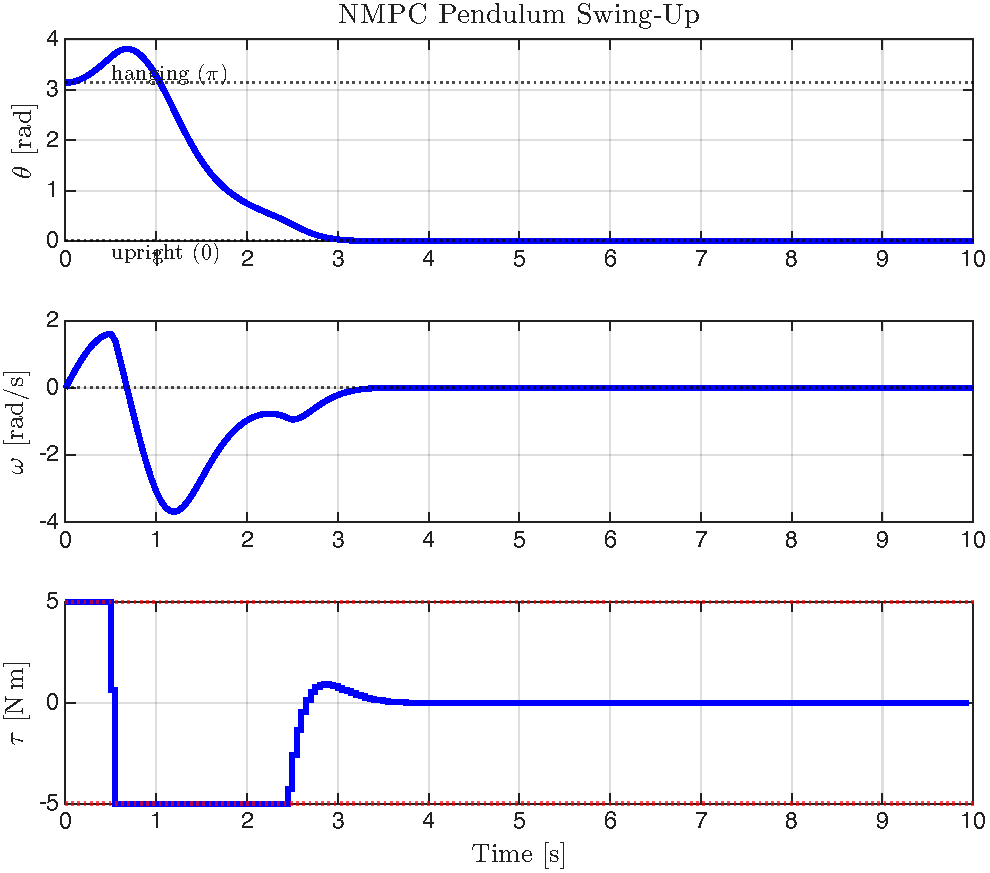
\includegraphics[width=0.85\textwidth]{Figures/fig_nmpc_pendulum_swingup.pdf}
	\caption{NMPC pendulum swing-up. Top: angle $\theta$ from the upright position ($\theta = \pi$ is hanging, $\theta = 0$ is inverted). The controller pumps energy by swinging through the lower equilibrium before catching the pendulum at the top. Middle: angular velocity $\omega$. Bottom: applied torque $\tau$, saturating at $\pm 5$\,N\,m during the swing phase.}
	\label{fig:nmpc_pendulum}
\end{figure}

\begin{notebox}{Alternative: fmincon for Readers Without CasADi}
	The same problem can be solved using MATLAB's \texttt{fmincon} with direct multiple shooting. Pack the decision variables as $z = [u_0, \dots, u_{N-1}, \theta_1, \omega_1, \dots, \theta_N, \omega_N]$, implement the RK4 dynamics as nonlinear equality constraints, and use the \texttt{'interior-point'} algorithm. CasADi is preferred because it provides exact derivatives automatically, whereas \texttt{fmincon} relies on finite differences (slower, less accurate). The figure-generation script \texttt{gen\_figures\_nmpc.m} accompanying this book uses \texttt{fmincon} so that no additional toolbox installation is required.
\end{notebox}


% ================================================================
% SEQUENTIAL CONVEX PROGRAMMING
% ================================================================
\section{Sequential Convex Programming}
\label{sec:scp}

NLP solvers (IPOPT, SNOPT) are general and powerful but carry overhead: algorithmic differentiation infrastructure, barrier parameter management, and convergence to local---not global---minima. For many NMPC problems, a more direct strategy exists: replace the non-convex NLP with a \emph{sequence of convex subproblems}, each of which is a QP or second-order cone programme (SOCP).

The key observation: at a given trajectory estimate $(\bar{x}, \bar{u})$, the nonlinear dynamics $f$ and any non-convex constraints can be \emph{linearised} to produce a convex approximation. Solving this approximation gives a better trajectory estimate, and the process repeats.

\subsection{From Chapter~\ref{chap:linear_mpc} Tracking to Iterative Refinement}

In Section~\ref{sec:tracking_mpc}, we linearised the robot dynamics around the \emph{reference trajectory} and solved a single QP per MPC step. This works when the actual state stays close to the reference. But what if the reference is unavailable, or the deviation is large?

\emph{Successive convexification} (SCvx) generalises this idea: linearise around the \emph{current best trajectory estimate}, solve the QP, update the estimate, and iterate until convergence. The reference trajectory is replaced by the previous iteration's solution.

\subsection{Successive Convexification (SCvx)}
\label{sec:scvx}

Given a trajectory estimate $(\bar{x}_0, \bar{u}_0, \dots, \bar{x}_N, \bar{u}_{N-1})$ from the previous iteration, linearise the dynamics at each time step:
\begin{align*}
	A_k &= \left.\frac{\partial f}{\partial x}\right|_{\bar{x}_k, \bar{u}_k}, &
	B_k &= \left.\frac{\partial f}{\partial u}\right|_{\bar{x}_k, \bar{u}_k}, &
	c_k &= f(\bar{x}_k, \bar{u}_k) - A_k\,\bar{x}_k - B_k\,\bar{u}_k.
\end{align*}
The \emph{affine approximation} of the dynamics is:
\[
x_{k+1} \approx A_k\, x_k + B_k\, u_k + c_k.
\]
Two mechanisms ensure convergence:

\begin{alertbox}{SCvx Is Not a Controller---It Is an Offline Trajectory Optimiser}
	SCvx solves the nonlinear OCP \emph{once} for a fixed initial condition $x_0$. It is not a receding-horizon controller. To use SCvx inside an MPC loop, one would run the full SCvx iteration (Steps~1--6 below) at each sampling instant---which is computationally expensive. The Real-Time Iteration scheme (Section~\ref{sec:rti}) addresses this by performing only \emph{one} SCvx iteration per time step.
\end{alertbox}

Two mechanisms ensure convergence of the iterative linearisation:

\textbf{Trust region.} The linearised dynamics $A_k x_k + B_k u_k + c_k$ are only accurate near the linearisation point $(\bar{x}_k, \bar{u}_k)$. A \emph{trust region} restricts the new trajectory to stay within a ball of radius $\Delta$ around the current estimate:
\[
\|x_k - \bar{x}_k\|_\infty \le \Delta, \qquad \|u_k - \bar{u}_k\|_\infty \le \Delta.
\]
Within this region, the linearisation error is controlled. After each iteration, $\Delta$ is adjusted based on how well the linearisation predicted the actual cost change (see Step~5 below).

\textbf{Virtual control.} Adding a slack variable $\nu_k \in \mathbb{R}^{n_x}$ to the linearised dynamics,
\[
x_{k+1} = A_k\, x_k + B_k\, u_k + c_k + \nu_k,
\]
and penalising $\|\nu_k\|_1 = \sum_i |\nu_{k,i}|$ (the $\ell_1$ norm, i.e.\ the sum of absolute values of all components) heavily in the cost ensures the subproblem is always feasible, even when the trust region is tight. At convergence, $\nu_k \to 0$ and the linearised dynamics match the true dynamics.

\begin{defnbox}{SCvx Algorithm}
	Given: nonlinear dynamics $f$, cost $\ell$, constraints $h$, initial state $x_0$, convergence tolerance $\varepsilon$.
	\begin{enumerate}[nosep]
		\item \textbf{Initialise:} Choose an initial trajectory guess $(\bar{x}^{(0)}, \bar{u}^{(0)})$ and trust-region radius $\Delta^{(0)}$. Set iteration counter $i = 0$.
		\item \textbf{Convexify:} At each time step $k = 0, \dots, N{-}1$, compute the Jacobians $A_k$, $B_k$ and the affine constant $c_k$ by linearising $f$ around $(\bar{x}_k^{(i)}, \bar{u}_k^{(i)})$.
		\item \textbf{Solve QP:} With the linearised dynamics and trust region fixed, solve the convex subproblem:
		\begin{align*}
			\min_{x, u, \nu} \quad & \sum_{k=0}^{N-1} \bigl[\ell(x_k, u_k) + w_\nu \|\nu_k\|_1\bigr] + V_f(x_N) \\
			\text{s.t.} \quad & x_{k+1} = A_k x_k + B_k u_k + c_k + \nu_k \\
			& h(x_k, u_k) \le 0 \;\;\text{(convex constraints kept exactly)} \\
			& \|x_k - \bar{x}_k^{(i)}\|_\infty \le \Delta^{(i)},\;\; \|u_k - \bar{u}_k^{(i)}\|_\infty \le \Delta^{(i)}
		\end{align*}
		Denote the solution $(x^*, u^*, \nu^*)$.
		\item \textbf{Evaluate actual cost:} Simulate the \emph{true} nonlinear dynamics $x_{k+1} = f(x_k, u_k^*)$ using the solved inputs $u^*$. Compute the \emph{actual} nonlinear cost $J_{\text{actual}}$. Also record the cost $J_{\text{model}}$ predicted by the convex subproblem.
		\item \textbf{Adjust trust region:} Compute the trust-region ratio
		\[
			\rho = \frac{J_{\text{prev}} - J_{\text{actual}}}{J_{\text{prev}} - J_{\text{model}}},
		\]
		where $J_{\text{prev}}$ is the actual nonlinear cost at the previous iterate $(\bar{x}^{(i)}, \bar{u}^{(i)})$. The ratio $\rho$ measures how well the linear model predicted the true cost change:
		\begin{itemize}[nosep]
			\item $\rho \approx 1$: the linear model was accurate $\;\Rightarrow\;$ increase $\Delta$ (e.g., $\Delta \leftarrow 2\Delta$) to allow larger steps.
			\item $0 < \rho \ll 1$: the model over-predicted the improvement $\;\Rightarrow\;$ keep $\Delta$ or decrease it.
			\item $\rho \le 0$: the actual cost \emph{increased} despite the model predicting a decrease $\;\Rightarrow\;$ reject the step (keep $\bar{x}^{(i)}, \bar{u}^{(i)}$) and shrink $\Delta$ (e.g., $\Delta \leftarrow \Delta/2$).
		\end{itemize}
		If the step is accepted, set $(\bar{x}^{(i+1)}, \bar{u}^{(i+1)}) \leftarrow (x^*, u^*)$. Otherwise, keep the previous iterate and re-solve with the smaller trust region.
		\item \textbf{Convergence:} Stop when both the trajectory change and virtual control are below tolerance:
		\[
			\max_k\|x_k^* - \bar{x}_k^{(i)}\| < \varepsilon \quad\text{and}\quad \max_k\|\nu_k^*\| < \varepsilon.
		\]
		Otherwise, set $i \leftarrow i + 1$ and return to Step~2.
	\end{enumerate}
\end{defnbox}

Each subproblem is a QP (if $\ell$ is quadratic and constraints are linear/quadratic) and can be solved with \texttt{quadprog}. The trust region and virtual control add $2(n_x + n_u)N + n_x N$ variables and constraints---modest overhead for a standard QP solver.

\begin{alertbox}{Convergence of SCvx}
	Under Lipschitz-continuity of $f$ and its Jacobians, SCvx converges superlinearly to a KKT point of the original non-convex problem~\cite{Mao2020}. The trust-region mechanism ensures each iteration decreases a merit function (the original cost plus a penalty on constraint violation), preventing divergence. In practice, 5--15 iterations typically suffice.
\end{alertbox}

\subsection{GUSTO: Penalised Trust Regions}
\label{sec:gusto}

\emph{GuSTO} (Guaranteed Sequential Trajectory Optimisation)~\cite{Bonalli2019} replaces the hard trust-region constraint with a soft penalty. At iteration $i$, solve:
\[
\min_{x, u, \nu} \;\; \sum_{k=0}^{N-1}\bigl[\ell(x_k, u_k) + w_\nu \|\nu_k\|_1\bigr] + V_f(x_N) + \frac{\lambda^{(i)}}{2}\sum_{k=0}^{N}\|x_k - \bar{x}_k^{(i)}\|^2
\]
subject to the same linearised dynamics and convex constraints, but \emph{without} the trust-region inequality.

The penalty weight $\lambda^{(i)}$ is adjusted automatically:
\begin{itemize}[nosep]
	\item Compute the \emph{actual} nonlinear cost $J_{\text{true}}$ at the new iterate.
	\item If $J_{\text{true}}$ decreased sufficiently relative to the predicted decrease, accept the step and reduce $\lambda$ (allow larger steps next iteration).
	\item Otherwise, reject the step and increase $\lambda$ (force smaller steps).
\end{itemize}

The advantage over SCvx: no trust-region constraint to manage, and the penalty parameter adapts without manual tuning. Under standard regularity assumptions, GuSTO converges to a KKT point of the original problem~\cite{Bonalli2019}.

\begin{summarybox}{SCvx vs.\ GuSTO}
	\begin{center}
		\renewcommand{\arraystretch}{1.3}
		\begin{tabular}{p{0.44\textwidth} p{0.44\textwidth}}
			\toprule
			\textbf{SCvx} & \textbf{GuSTO} \\
			\midrule
			Hard trust region $\|x - \bar{x}\|_\infty \le \Delta$ & Soft penalty $\lambda\|x - \bar{x}\|^2$ in cost \\
			Trust-region radius $\Delta$ updated by ratio test & Penalty weight $\lambda$ updated by step acceptance \\
			Subproblem has extra inequality constraints & Subproblem has modified cost only \\
			Superlinear convergence guarantee & Convergence guarantee under milder assumptions \\
			Widely used in aerospace (powered landing) & Simpler implementation \\
			\bottomrule
		\end{tabular}
	\end{center}
\end{summarybox}


% ================================================================
% ROCKET LANDING
% ================================================================
\section{Application: Powered Descent Guidance}
\label{sec:rocket_landing}

Powered descent guidance---steering a rocket to a soft landing---is a flagship application of sequential convex programming. The problem is inherently nonlinear (thrust direction is coupled to vehicle attitude through trigonometric functions), subject to hard constraints (thrust limits, tilt angle, ground plane), and must be solved reliably under tight computational budgets.

\subsection{The Rocket Model}

Consider a planar (2D) rocket with state $x = [p_x,\; p_y,\; v_x,\; v_y,\; \theta,\; \omega]^\top$ and input $u = [T,\; \delta]^\top$:

\begin{center}
\renewcommand{\arraystretch}{1.2}
\begin{tabular}{cl|cl}
	\toprule
	\textbf{State} & \textbf{Description} & \textbf{Input} & \textbf{Description} \\
	\midrule
	$p_x, p_y$ & position [m] & $T$ & thrust magnitude [N] \\
	$v_x, v_y$ & velocity [m/s] & $\delta$ & gimbal angle [rad] \\
	$\theta$ & tilt from vertical [rad] & & \\
	$\omega$ & angular rate [rad/s] & & \\
	\bottomrule
\end{tabular}
\end{center}

The continuous-time dynamics are:
\begin{align*}
	\dot{p}_x &= v_x, &
	\dot{p}_y &= v_y, \\
	\dot{v}_x &= -\frac{T}{m}\sin(\theta + \delta), &
	\dot{v}_y &= \frac{T}{m}\cos(\theta + \delta) - g, \\
	\dot{\theta} &= \omega, &
	\dot{\omega} &= -\frac{T\,\ell}{J}\sin(\delta),
\end{align*}
where $m$ is the rocket mass, $g$ gravitational acceleration, $J$ the moment of inertia, and $\ell$ the distance from the centre of gravity to the engine nozzle. The gimbal angle $\delta$ deflects the thrust vector relative to the body axis; the resulting lateral force component creates a torque about the centre of gravity.

\textbf{Discretisation.} Applying Forward Euler with step size $T_s$:
\begin{equation*}
	x_{k+1} = f(x_k, u_k) =
	\begin{bmatrix}
		p_{x,k} + T_s\, v_{x,k} \\
		p_{y,k} + T_s\, v_{y,k} \\
		v_{x,k} - T_s\,\frac{T_k}{m}\sin(\theta_k + \delta_k) \\
		v_{y,k} + T_s\!\left(\frac{T_k}{m}\cos(\theta_k + \delta_k) - g\right) \\
		\theta_k + T_s\, \omega_k \\
		\omega_k - T_s\,\frac{T_k\,\ell}{J}\sin(\delta_k)
	\end{bmatrix}.
\end{equation*}

\textbf{Jacobians.} At a linearisation point $(\bar{x}_k, \bar{u}_k)$ with $\bar{\theta} = \bar{x}_{5,k}$, $\bar{T} = \bar{u}_{1,k}$, $\bar{\delta} = \bar{u}_{2,k}$:
\[
A_k = \begin{bmatrix}
	1 & 0 & T_s & 0 & 0 & 0 \\
	0 & 1 & 0 & T_s & 0 & 0 \\
	0 & 0 & 1 & 0 & -\frac{T_s \bar{T}}{m}\cos(\bar{\theta}+\bar{\delta}) & 0 \\
	0 & 0 & 0 & 1 & -\frac{T_s \bar{T}}{m}\sin(\bar{\theta}+\bar{\delta}) & 0 \\
	0 & 0 & 0 & 0 & 1 & T_s \\
	0 & 0 & 0 & 0 & 0 & 1
\end{bmatrix},
\]
\[
B_k = \begin{bmatrix}
	0 & 0 \\
	0 & 0 \\
	-\frac{T_s}{m}\sin(\bar{\theta}+\bar{\delta}) & -\frac{T_s \bar{T}}{m}\cos(\bar{\theta}+\bar{\delta}) \\[3pt]
	\frac{T_s}{m}\cos(\bar{\theta}+\bar{\delta}) & -\frac{T_s \bar{T}}{m}\sin(\bar{\theta}+\bar{\delta}) \\[3pt]
	0 & 0 \\
	-\frac{T_s \ell}{J}\sin(\bar{\delta}) & -\frac{T_s \bar{T}\ell}{J}\cos(\bar{\delta})
\end{bmatrix}.
\]

\subsection{Constraints}

\begin{itemize}[nosep]
	\item \textbf{Thrust bounds:} $T_{\min} \le T_k \le T_{\max}$. Rocket engines cannot throttle below a minimum level; they are either off or above $T_{\min}$.
	\item \textbf{Gimbal limit:} $|\delta_k| \le \delta_{\max}$. The nozzle has a finite range of motion.
	\item \textbf{Tilt limit:} $|\theta_k| \le \theta_{\max}$. Large tilt angles risk loss of control and are structurally dangerous.
	\item \textbf{Ground plane:} $p_{y,k} \ge 0$. The rocket must stay above the landing surface.
	\item \textbf{Terminal conditions:} $x_N = [0,\; 0,\; 0,\; 0,\; 0,\; 0]^\top$ (soft landing at the target with zero velocity and zero tilt).
\end{itemize}

The thrust bounds, gimbal limit, tilt limit, and ground plane constraints are all convex (they are linear in the decision variables). These are kept exactly in the SCvx subproblem---only the dynamics are linearised.

\begin{alertbox}{The Non-Convexity of Thrust Lower Bounds}
	If the input were a 2D thrust vector $T = [T_x, T_y]^\top$, the constraint $T_{\min} \le \|T\| \le T_{\max}$ would be non-convex (the feasible region is an annulus). \emph{Lossless convexification}~\cite{Acikmese2007} shows that this non-convex constraint can be relaxed to the convex pair $T_{\min} \le \Gamma$, $\|T\| \le \Gamma$ without changing the optimal solution. In our formulation, using scalar thrust $T$ with $T_{\min} \le T \le T_{\max}$ avoids this issue entirely---the constraint is already a simple bound.
\end{alertbox}

\subsection{SCvx Formulation for Rocket Landing}

The objective is fuel-optimal landing: minimise total impulse $\sum_{k=0}^{N-1} T_k\, T_s$. At SCvx iteration $i$, the subproblem is:
\begin{align*}
	\min_{x, u, \nu} \quad & \sum_{k=0}^{N-1} \bigl[T_s\, T_k + w_\nu \|\nu_k\|_1\bigr] \\[4pt]
	\text{s.t.} \quad
	& x_{k+1} = A_k^{(i)}\, x_k + B_k^{(i)}\, u_k + c_k^{(i)} + \nu_k \\
	& T_{\min} \le T_k \le T_{\max}, \quad |\delta_k| \le \delta_{\max} \\
	& |\theta_k| \le \theta_{\max}, \quad p_{y,k} \ge 0 \\
	& \|x_k - \bar{x}_k^{(i)}\|_\infty \le \Delta^{(i)} \\
	& x_0 = x_{\text{init}}, \quad x_N = x_{\text{final}}
\end{align*}

The $\|\nu_k\|_1$ penalty is reformulated using auxiliary variables: $\nu_k^+ - \nu_k^- = \nu_k$, $\nu_k^+, \nu_k^- \ge 0$, and the penalty becomes $w_\nu \sum (\nu_k^+ + \nu_k^-)$. This keeps the subproblem as a linear programme (LP) or, if a quadratic trust-region penalty is used, a QP.

\subsection{MATLAB Implementation}

The following code implements SCvx for the rocket landing using YALMIP and \texttt{quadprog}.

\begin{lstlisting}[language=Matlab, caption={SCvx for powered descent guidance (rocket landing).}, label=lst:scvx_rocket]
% Parameters
m = 30; g_val = 9.81; J_r = 10; l_arm = 1.5;
Ts = 0.2; N_h = 40; nx = 6; nu = 2;
T_min = 40; T_max = 400;
del_max = 0.35;  th_max = 0.785;  % 20 deg, 45 deg
w_vc = 1e5;      % virtual control penalty

x0 = [12; 50; -2; -10; 0.05; 0];
xf = zeros(6, 1);

% Nonlinear dynamics (Forward Euler)
f_nl = @(x, u) [x(1) + Ts*x(3);
                 x(2) + Ts*x(4);
                 x(3) - Ts*(u(1)/m)*sin(x(5)+u(2));
                 x(4) + Ts*((u(1)/m)*cos(x(5)+u(2)) - g_val);
                 x(5) + Ts*x(6);
                 x(6) - Ts*(u(1)*l_arm/J_r)*sin(u(2))];

% Initial guess: linear interpolation + hover thrust
xb = zeros(nx, N_h+1);  ub = zeros(nu, N_h);
for k = 0:N_h
    xb(:,k+1) = x0 + (k/N_h)*(xf - x0);
end
ub(1,:) = m * g_val;  % hover thrust

% SCvx iterations
max_iter = 15; Delta = 50; tol = 1e-3;
for iter = 1:max_iter
    % Compute Jacobians and affine terms at linearisation point
    Ak = zeros(nx, nx, N_h); Bk = zeros(nx, nu, N_h);
    ck = zeros(nx, N_h);
    for k = 1:N_h
        [Ak(:,:,k), Bk(:,:,k), ck(:,k)] = ...
            linearise(xb(:,k), ub(:,k), f_nl, Ts, m, g_val, J_r, l_arm);
    end

    % Solve QP subproblem
    x_var = sdpvar(nx, N_h+1, 'full');
    u_var = sdpvar(nu, N_h, 'full');
    nu_vc = sdpvar(nx, N_h, 'full');

    con = [x_var(:,1) == x0, x_var(:,N_h+1) == xf];
    obj = 0;
    for k = 1:N_h
        con = [con, x_var(:,k+1) == Ak(:,:,k)*x_var(:,k) ...
               + Bk(:,:,k)*u_var(:,k) + ck(:,k) + nu_vc(:,k)];
        con = [con, T_min <= u_var(1,k) <= T_max];
        con = [con, -del_max <= u_var(2,k) <= del_max];
        con = [con, -th_max <= x_var(5,k) <= th_max];
        con = [con, x_var(2,k) >= 0];
        % Trust region
        con = [con, -Delta <= x_var(:,k)-xb(:,k) <= Delta];
        con = [con, -Delta <= u_var(:,k)-ub(:,k) <= Delta];
        obj = obj + Ts*u_var(1,k) + w_vc*norm(nu_vc(:,k),1);
    end
    optimize(con, obj, sdpsettings('verbose',0,'solver','quadprog'));

    x_new = value(x_var); u_new = value(u_var);
    vc_norm = max(abs(value(nu_vc(:))));
    dx = max(abs(x_new(:) - xb(:)));

    fprintf('Iter %2d: dx=%.4e, vc=%.4e\n', iter, dx, vc_norm);
    xb = x_new; ub = u_new;
    if dx < tol && vc_norm < tol, break; end
end
\end{lstlisting}

The \texttt{linearise} helper computes the Jacobians $A_k$, $B_k$ and the constant $c_k = f(\bar{x}_k, \bar{u}_k) - A_k \bar{x}_k - B_k \bar{u}_k$ at each time step using the analytical expressions derived above:

\begin{lstlisting}[language=Matlab, caption={The \texttt{linearise} helper function for the rocket dynamics.}, label=lst:linearise_helper]
function [Ak, Bk, ck] = linearise(xb, ub, f_nl, Ts, m, g_val, J_r, l_arm)
    th = xb(5); T_b = ub(1); del = ub(2);
    s = sin(th + del); c = cos(th + del);
    Ak = [1 0 Ts 0  0 0;
          0 1 0  Ts 0 0;
          0 0 1  0  -Ts*T_b/m*c  0;
          0 0 0  1  -Ts*T_b/m*s  0;
          0 0 0  0   1           Ts;
          0 0 0  0   0            1];
    Bk = [0              0;
          0              0;
         -Ts/m*s        -Ts*T_b/m*c;
          Ts/m*c        -Ts*T_b/m*s;
          0              0;
         -Ts*l_arm/J_r*sin(del)  -Ts*T_b*l_arm/J_r*cos(del)];
    ck = f_nl(xb, ub) - Ak*xb - Bk*ub;
end
\end{lstlisting}

\begin{notebox}{Figures Generated with GuSTO Variant}
	The figures in this section were generated using the GuSTO variant (soft quadratic proximity penalty, no hard trust region), which is described in Section~\ref{sec:gusto}. Both SCvx and GuSTO converge to the same optimal trajectory for this problem; the GuSTO variant was used because it proved more robust to the initial guess.
\end{notebox}

\subsection{Results}

Figure~\ref{fig:nmpc_rocket_traj} shows the landing trajectory computed by SCvx. The rocket starts at $(12,\; 50)$\,m with downward velocity $v_y = -10$\,m/s and a slight horizontal drift. The trajectory change $\max_k\|x_k^{(i+1)} - x_k^{(i)}\|_\infty$ decreases monotonically from $\sim 20$ to below $0.1$ within 15 iterations (Figure~\ref{fig:scvx_convergence}), with virtual control magnitude at machine precision throughout. The converged trajectory is fuel-optimal subject to all constraints.

The landing sequence proceeds in three phases:
\begin{enumerate}[nosep]
	\item \textbf{Gravity turn}: the rocket tilts to cancel horizontal velocity while gravity decelerates the vertical motion.
	\item \textbf{Braking burn}: thrust increases to decelerate the descent.
	\item \textbf{Final approach}: the rocket is nearly vertical, decelerating smoothly to zero velocity at the surface.
\end{enumerate}

\begin{figure}[ht]
	\centering
	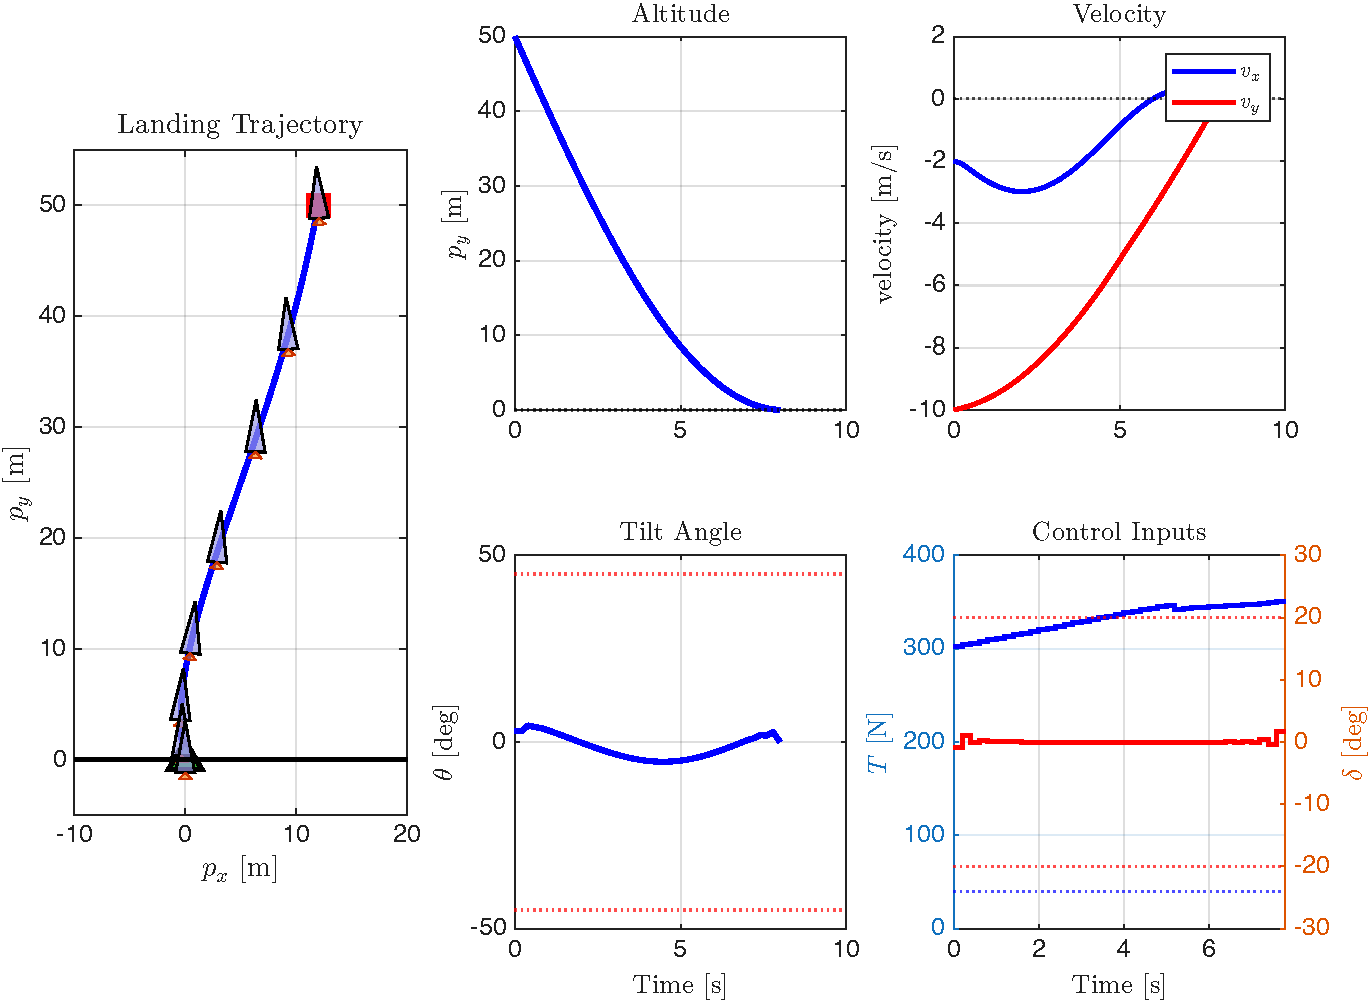
\includegraphics[width=0.9\textwidth]{Figures/fig_nmpc_rocket_traj.pdf}
	\caption{Rocket landing trajectory computed by SCvx. Left: 2D trajectory with rocket attitude at selected time steps. The rocket corrects horizontal drift, decelerates, and lands vertically at the target. Right, top to bottom: altitude, velocity components, tilt angle, and thrust/gimbal inputs. Dashed lines indicate constraint limits.}
	\label{fig:nmpc_rocket_traj}
\end{figure}

\begin{figure}[ht]
	\centering
	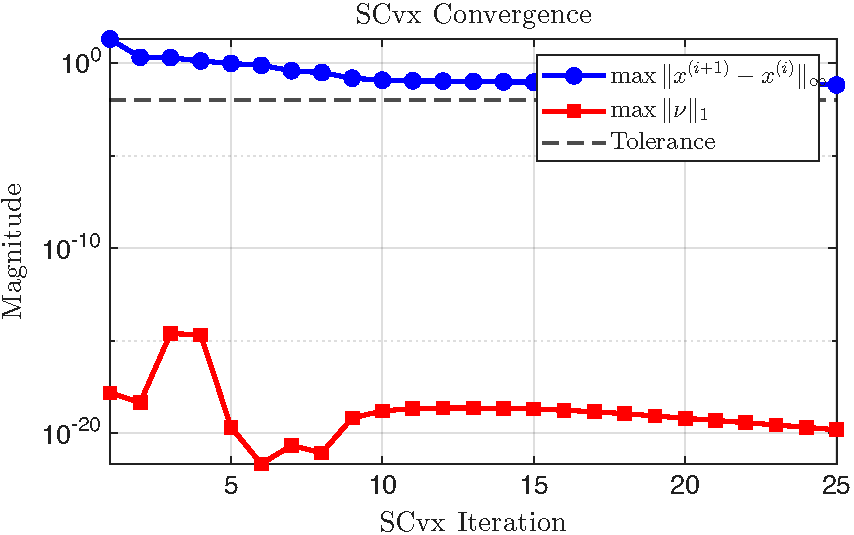
\includegraphics[width=0.7\textwidth]{Figures/fig_scvx_convergence.pdf}
	\caption{SCvx convergence: maximum trajectory change $\max_k\|x_k^{(i+1)} - x_k^{(i)}\|_\infty$ and virtual control magnitude $\max_k\|\nu_k\|_1$ versus iteration. Both quantities decrease below the tolerance $10^{-3}$ within approximately 10 iterations.}
	\label{fig:scvx_convergence}
\end{figure}


% ================================================================
% REAL-TIME NMPC
% ================================================================
\section{Real-Time Nonlinear MPC}
\label{sec:rt_nmpc}

In a receding-horizon loop, the NLP (or SCP sequence) must be solved within one sampling period $T_s$. For fast systems ($T_s$ in the millisecond range), this is the primary bottleneck.

\subsection{The Real-Time Iteration (RTI)}
\label{sec:rti}

The \emph{Real-Time Iteration} scheme~\cite{Diehl2005} exploits the fact that consecutive MPC problems differ only slightly (the state has moved by one step). Instead of solving each NLP to convergence, RTI performs a \emph{single SQP iteration} per sampling instant:

\begin{enumerate}[nosep]
	\item \textbf{Preparation phase} (between samples): linearise the dynamics and form the QP using the \emph{shifted} previous solution as the reference trajectory.
	\item \textbf{Feedback phase} (at the sampling instant): update the initial state $x_0 = x(t)$, solve the QP, and apply $u_0^*$.
\end{enumerate}

The feedback phase involves only a QP solve---typically microseconds to milliseconds for structured solvers. Over successive time steps, the single-iteration updates accumulate into full NLP convergence, provided the system evolves continuously. RTI is the workhorse of real-time NMPC and is implemented in the \emph{acados} framework~\cite{Verschueren2022}.

\begin{notebox}{RTI and Successive Linearisation}
	RTI is closely related to the successive linearisation of Section~\ref{sec:tracking_mpc}: both perform one linearisation and one QP solve per time step. The difference is that RTI linearises around the \emph{shifted previous solution} (which tracks the actual trajectory), whereas successive linearisation in Section~\ref{sec:tracking_mpc} uses the \emph{known reference trajectory}. RTI is more general---it does not require a reference.
\end{notebox}

\subsection{Warm-Starting and Shifted Initialisation}

At time $t$, the previous solution provides a trajectory $x_0^*, x_1^*, \dots, x_N^*$ and controls $u_0^*, u_1^*, \dots, u_{N-1}^*$. The \emph{shifted initialisation} for the next time step is:
\[
\bar{x}_k^{\text{new}} = x_{k+1}^*, \;\; k = 0, \dots, N{-}1, \qquad \bar{x}_N^{\text{new}} = f(x_N^*, u_{N-1}^*),
\]
\[
\bar{u}_k^{\text{new}} = u_{k+1}^*, \;\; k = 0, \dots, N{-}2, \qquad \bar{u}_{N-1}^{\text{new}} = u_{N-1}^*.
\]
This provides an excellent initial guess for the NLP solver (or SCvx), dramatically reducing the number of iterations needed.


% ================================================================
% PRACTICAL GUIDELINES
% ================================================================
\section{Practical Guidelines}
\label{sec:nmpc_guidelines}

\begin{summarybox}{Comparison of NMPC Solution Methods}
	\begin{center}
		\renewcommand{\arraystretch}{1.3}
		\begin{tabular}{p{0.16\textwidth} p{0.16\textwidth} p{0.16\textwidth} p{0.16\textwidth} p{0.16\textwidth}}
			\toprule
			& \textbf{Full NLP} & \textbf{SCvx} & \textbf{GuSTO} & \textbf{RTI} \\
			\midrule
			\textbf{Subproblem} & NLP (IPOPT) & QP/SOCP & QP & QP \\
			\textbf{Iterations} & To convergence & 5--15 & 5--15 & 1 per step \\
			\textbf{Tools} & CasADi & YALMIP/CVX & YALMIP/CVX & acados \\
			\textbf{Guarantees} & Local NLP & KKT point & KKT point & Asymptotic \\
			\textbf{Computation} & ms--s & $<$ ms each & $<$ ms each & $\mu$s--ms \\
			\textbf{Best for} & Offline / slow & Trajectory opt. & Trajectory opt. & Real-time \\
			\bottomrule
		\end{tabular}
	\end{center}
\end{summarybox}

\textbf{When to use what:}
\begin{itemize}[nosep]
	\item \textbf{Small system, slow dynamics} ($T_s > 100$\,ms): Full NLP via CasADi/IPOPT is the simplest and most flexible.
	\item \textbf{Trajectory optimisation} (offline planning): SCvx or GuSTO. The QP subproblems are fast and the convergence is reliable.
	\item \textbf{Fast dynamics} ($T_s < 10$\,ms): RTI with acados. One QP per step, microsecond feedback.
	\item \textbf{Safety-critical}: SCvx or GuSTO with convergence verification. The convex subproblems have certified solvers and no risk of converging to a poor local minimum of the subproblem.
\end{itemize}


% ================================================================
% SUMMARY
% ================================================================
\section*{Summary}

\begin{summarybox}{Nonlinear MPC}
	\begin{enumerate}[nosep]
		\item NMPC replaces linear dynamics $Ax + Bu$ with the full nonlinear model $f(x, u)$. The resulting optimisation is a non-convex NLP.
		\item \textbf{Direct multiple shooting} is the standard transcription: both states and controls are decision variables, dynamics are equality constraints, and the NLP has exploitable sparsity.
		\item \textbf{CasADi + IPOPT} provides a complete NLP workflow with automatic differentiation. Suitable for offline or slow real-time applications.
		\item \textbf{Sequential convex programming} (SCvx, GuSTO) replaces the NLP with a sequence of QPs by linearising the dynamics at each iteration. Trust regions or penalty terms ensure convergence.
		\item \textbf{Real-Time Iteration} performs one SQP/QP step per sampling instant, enabling NMPC at millisecond rates.
		\item The choice of method depends on the sampling rate, system size, and certification requirements.
	\end{enumerate}
\end{summarybox}


% ================================================================
% EXERCISES
% ================================================================
\section*{Exercises}
\begin{enumerate}

\item \textbf{(Direct Multiple Shooting for a Van der Pol Oscillator)}
Consider the Van der Pol oscillator:
\[
\dot{x}_1 = x_2, \qquad \dot{x}_2 = \mu(1 - x_1^2)\,x_2 - x_1 + u,
\]
with $\mu = 1$, $|u| \le 1$, $T_s = 0.1$\,s, $N = 20$.
\begin{enumerate}
	\item Discretise using Forward Euler. Write out the nonlinear discrete-time equations.
	\item Formulate the direct multiple shooting NLP for driving $x_0 = [2;\; 0]$ to the origin with cost $\sum x_k^\top I\, x_k + 0.1\, u_k^2$. State all decision variables and constraints.
	\item Implement in MATLAB using \texttt{fmincon}. Plot the resulting state and control trajectories. Does the solver converge from a zero initial guess?
	\item Compare the solution obtained from two different initial guesses. Does the NLP have multiple local minima?
\end{enumerate}

\item \textbf{(SCvx for Nonlinear Path Planning)}
A point mass in 2D with state $x = [p_x,\; p_y,\; v_x,\; v_y]^\top$ and input $u = [a_x,\; a_y]^\top$ has linear dynamics $\dot{p} = v$, $\dot{v} = u$, with $\|u\|_2 \le a_{\max}$. An obstacle at position $p_{\text{obs}}$ with radius $r_{\text{obs}}$ imposes the non-convex constraint $\|p_k - p_{\text{obs}}\|_2 \ge r_{\text{obs}}$.
\begin{enumerate}
	\item Show that the obstacle avoidance constraint is non-convex.
	\item Linearise the obstacle constraint at a point $\bar{p}_k$ to obtain a halfspace approximation. Write out the resulting linear inequality.
	\item Implement SCvx in MATLAB/YALMIP with $a_{\max} = 2$, $p_{\text{obs}} = [5;\; 0]$, $r_{\text{obs}} = 2$, initial state $(0, 0, 1, 0)$, target $(10, 0, 0, 0)$, $N = 40$, $T_s = 0.2$\,s. Plot the trajectory at iterations 1, 3, 5, and convergence.
	\item What happens if the initial trajectory guess passes through the obstacle? Does SCvx still converge?
\end{enumerate}

\item \textbf{(Rocket Landing: Sensitivity Analysis)}
Using the rocket model from Section~\ref{sec:rocket_landing} with the parameters given:
\begin{enumerate}
	\item Modify the initial horizontal offset to $p_{x,0} = 0$ (directly above the target). How does the optimal trajectory change? Does the rocket still need to tilt?
	\item Increase the minimum thrust to $T_{\min} = 100$\,N. How does this affect the descent profile? At what $T_{\min}$ does the problem become infeasible?
	\item Replace the fuel-optimal cost ($\min \sum T_k$) with a time-optimal cost. Formulate the modified problem and discuss the challenges of free-final-time optimisation in the SCvx framework.
\end{enumerate}

\item \textbf{(Comparing SCvx and GuSTO)}
Implement both SCvx (with trust region $\Delta = 50$) and GuSTO (with initial penalty $\lambda = 0.1$) for the rocket landing problem.
\begin{enumerate}
	\item Plot the number of iterations to convergence for each method as a function of the initial trajectory guess quality (vary the initial guess from ``poor'' --- constant hover thrust --- to ``good'' --- a preliminary trajectory from a coarser discretisation).
	\item Compare the final cost (total fuel) achieved by each method. Are they the same?
	\item Which method is more sensitive to the initial guess?
\end{enumerate}

\item \textbf{(Real-Time Iteration for a Nonlinear System)}
Consider the pendulum from Section~\ref{sec:nmpc_nlp} in a receding-horizon loop.
\begin{enumerate}
	\item Implement the full NMPC controller (solving the NLP to convergence at each step using \texttt{fmincon} or CasADi). Record the computation time per step.
	\item Implement RTI: at each step, perform a single SCvx iteration using the shifted previous solution. Record the computation time.
	\item Compare the closed-loop trajectories. For what initial conditions do the two approaches produce different results? Discuss the trade-off between computation time and optimality.
\end{enumerate}

\item \textbf{(Lossless Convexification)}
Consider a point-mass rocket in 2D with state $x = [p_x,\; p_y,\; v_x,\; v_y]^\top$ and thrust vector $T = [T_x,\; T_y]^\top$ (the input is the 2D thrust directly, not magnitude/angle). The constraint is $T_{\min} \le \|T\| \le T_{\max}$.
\begin{enumerate}
	\item Show that the constraint $T_{\min} \le \|T\|$ is non-convex by sketching the feasible set in $(T_x, T_y)$ space.
	\item The \emph{lossless convexification} relaxation introduces a slack variable $\Gamma$ and replaces the constraint with: $\|T\| \le \Gamma$, $T_{\min} \le \Gamma \le T_{\max}$. Show that this feasible set is convex.
	\item Argue (intuitively or formally) that at the optimum of a fuel-minimisation problem ($\min \sum \Gamma_k$), the relaxation is \emph{tight}: $\|T^*_k\| = \Gamma^*_k$. Why would the optimiser never waste fuel by having $\|T_k\| < \Gamma_k$?
\end{enumerate}

\end{enumerate}
